\section{Antenna Modelization}
The goal of this project is to develop an antenna that is compatible with 
WiFi standards (i.e. emits at $f=2.45\,\unit{GHz}$) and easily integrated
to textile. These two requirements impose multiple restrictions on both
the materials that can be used and the geometry of the antenna. For seamless
integration, we would like the antenna to be spun directly into the textile. 

Most solutions today merely affix a patch antenna to a less 
encumbered part of the textile, e.g. on the should pads of a shirt
or the front of a t-shirt.
A metallic plate shields the user from the electronic components 
of the patch antenna. Because the properties of patch antennas are
well known, it requires very little engineering and is thus cheap. However, integration 
with the textile is far from seamless, as it is very apparent to the
user that he has become a giant walking antenna. Our project thus 
strives to find antenna designs that have emission properties
as flexible as a patch antenna's while improving textile integration
as to make it become transparent to the user.

The concept of a fibre-antenna rapidly established itself
as an ideal solution in the research group. It provides a rich
architecture upon which to build. Moreover, it can easily 
be spun into textile as it can loaded into the spools that 
deliver threads to looms. Its mechanical properties make it
fit for daily use as it can resist a trip in the washing machine. 
Integration of the electronic components inside that fibre 
serves to shield both the user and the components. 

\begin{figure}
  \centering
  \begin{subfigure}[b]{\textwidth}
    \centering
   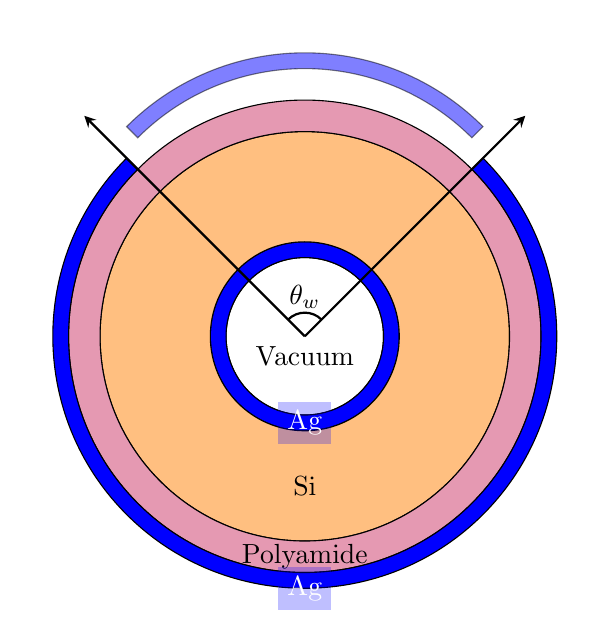
\begin{tikzpicture}
    % -- Draw different materials of the antenna.
    \coordinate (O) at (0,0);
    \draw (O) circle (1);											% Vacuum core
    \draw[fill=blue, even odd rule] (O) circle (1.2) (0:1) arc (0:360:1);					% Silver layer
    \draw[fill=orange!50!white, even odd rule] (O) circle (2.6) (0:1.2) arc (0:360:1.2);			% Dielectric (Si) layer
    \draw[fill=purple!40!white, even odd rule] (O) circle (3) (0:2.6) arc (0:360:2.6);				% Dielectric (polyamide) layer
    \draw[fill=blue,even odd rule] (45:3) -- (45:3.2) arc (45:-225:3.2) -- (-225:3) arc (-225:45:3) -- cycle;	% Second silver layer
    \draw[fill=blue,opacity=0.5,even odd rule,yshift=0.4cm] (45:3) -- (45:3.2) arc (45:135:3.2) -- (135:3) arc (135:45:3) -- cycle;
    
    % -- Draw the angular size of the window.
    \draw[->,>=stealth,thick] (O) -- (-2.8,2.8);
    \draw[->,>=stealth,thick] (O) -- (2.8,2.8);
    \draw[thick] (45:0.3) arc (45:135:.3); 
    \node at (0,0.5) {$\theta_w$};
    
    % -- Place text for materials
    \node at (0,-0.25) {Vacuum};
    \node[text=white,fill=blue,fill opacity=0.25,text opacity=1] at (0,-1.1) {Ag};
    \node at (0,-1.9) {Si};
    \node at (0,-2.8) {Polyamide};
    \node[text=white,fill=blue,fill opacity=0.25,text opacity=1] at (0,-3.2) {Ag};
   \end{tikzpicture}
   \vspace{0.25cm}
   \caption{View of the cross-section: in order of increasing radius, we have: vacuum, silver, silica, polyamide and silver.
	    We have shown a cross-section where there is a ``window''. When there are no windows, 
	    the outer silver layer takes up the entire circumference of the fiber.
	    $\theta_w$ is the angular size of the windows.}
   \label{fig:antenna.fibre-antenna.xsection}
  \end{subfigure}
  
  \vspace{2cm}
  
  \begin{subfigure}[b]{\textwidth}
    \centering
   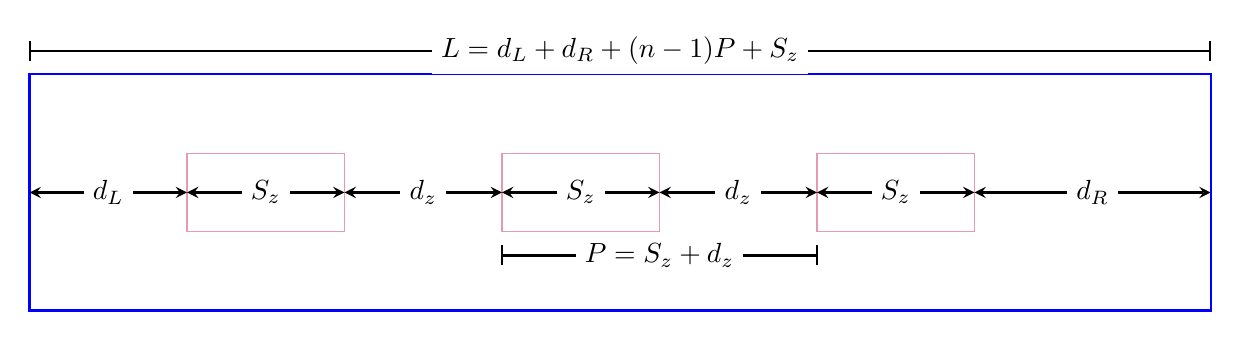
\begin{tikzpicture}
    \draw[blue,thick] (0,-0.5) rectangle (15,2.5);
    \draw[purple!40!white] (2,0.5) rectangle (4,1.5);
    \draw[purple!40!white] (6,0.5) rectangle (8,1.5);
    \draw[purple!40!white] (10,0.5) rectangle (12,1.5);
    
    \draw[<->,>=stealth,thick] (0,1) -- (2,1) node[midway,fill=white] {$d_L$};
    \draw[<->,>=stealth,thick] (2,1) -- (4,1) node[midway,fill=white] {$S_z$};
    \draw[<->,>=stealth,thick] (4,1) -- (6,1) node[midway,fill=white] {$d_z$};
    \draw[<->,>=stealth,thick] (6,1) -- (8,1) node[midway,fill=white] {$S_z$};
    \draw[<->,>=stealth,thick] (8,1) -- (10,1) node[midway,fill=white] {$d_z$};
    \draw[<->,>=stealth,thick] (10,1) -- (12,1) node[midway,fill=white] {$S_z$};
    \draw[<->,>=stealth,thick] (12,1) -- (15,1) node[midway,fill=white] {$d_R$};
    \draw[|-|,thick] (-0.01,2.8) -- (15.01,2.8) node[midway,fill=white] {$L=d_L+d_R+(n-1)P+S_z$};
    \draw[|-|,thick] (5.99,0.2) -- (10.01,0.2) node[midway,fill=white] {$P=S_z+d_z$};
   \end{tikzpicture}
   \vspace{0.25cm}
   \caption{Top view: the positions of the windows are usually asymmetric, i.e. $d_L\neq d_R$. The distance between
	    the windows is given by $d_z$ and the length of the windows are $S_z$. We notice that the length of the 
	    fibre is given by $L=d_L+d_R+(n-1)P+S_z$ where $P=S_z+d_z$ is the period between windows and $n$ is the number
	    of windows.}
   \label{fig:antenna.fibre-antenna.topview}
  \end{subfigure}
  \caption{Geometry of the fibre-antenna}
  \label{fig:antenna.fibre-antenna}
\end{figure}

\subsection{Leaky Coaxial Cable}
The first design we have looked into is a well known one:
the \textit{leaky coaxial fibre} (LCXF). It simply consists of
a coaxial cable (metal rod, dielectric layer, metal coating)
from which we have removed some of the metallic coating. 
These holes in the metallic coating are called ``windows'' and
allow light to escape the confines of the coax cable, hence
the moniker \textit{leaky}. In the following section, we will
look at several methods that we used to model the device
and present the design parameters that were used. 

\subsubsection{Specifications of the Devices}
An image is worth a thousand words. Figure \ref{fig:antenna.fibre-antenna.xsection}
shows a cross-section of the fibre. Figure \ref{fig:antenna.fibre-antenna.topview} 
shows a top view of the antenna and display the positions of the windows. 
Multiple designs have been fabricated, but we retain only those that 
we have tried to simulate. Table \ref{tab:antenna.rfxx-parameters} 
shows the actual geometrical parameters of the fibre-antennas.

\paragraph*{On the thickness of the silver shells}
The thicknesses of the dilectric materials are provided by the manufacturer, 
Polymicro Technologies, safe for the thicknesses of the silver layers. 
For the time being, we have calculated those thicknesses by measuring
the DC resistance of the inner and outer layers of silver and
using the relation \cite[p.~204]{CHE1989}
  \begin{equation}
    \label{eq:antenna.dcResistivity}
    R = \frac{L}{\sigma A}
  \end{equation}
where $L$ is the length of the fibre, $\sigma$ the conductivity of the silver
layer and $A$ its area. For the inner and outer layers, we have
  \begin{align}
    A_\text{inner}	&= \int_0^{2\pi}\int_{t_\text{vac}}^{t_\text{vac}+t_\text{Ag1}}r\,dr d\theta= \pi\left(2t_\text{vac}t_\text{Ag1}+t_\text{Ag1}^2\right)	\\
    A_\text{outer}	&= \int_0^{2\pi}\int_T^{T+t_\text{Ag2}}r\,dr d\theta = \pi\left(2Tt_\text{Ag2}+t_\text{Ag2}^2\right)
  \end{align}
where $T=t_\text{vac}+t_\text{Ag1}+t_\text{Si}+t_\text{pyamide}$. 
Substituting these results into \eqref{eq:antenna.dcResistivity}
yields
  \begin{subequations}
  \label{eq:antenna:thickGeneralEquations}
  \begin{align}  
   t_\text{Ag1}^2 + 2t_\text{vac}t_\text{Ag1}-\frac{L}{\sigma_\text{Ag0}\pi R_\text{inner}}	&=0	\\
   t_\text{Ag2}^2 + 2Tt_\text{Ag2}-\frac{L}{\sigma_\text{Ag0}\pi R_\text{outer}}			&=0
  \end{align}
  \end{subequations}
where the $R$s are the measured D.C. resistances measured for each shell. 
This can readily be solved using the quadratic equation. Using the bulk conductivity
of silver (see Table \ref{tab:antenna.physicalParameters}) yields the 
thicknesses found in Table \ref{tab:antenna.rfxx-parameters}.

In our previous simulations, it was clear that something was amiss:
there was no correlation between the simulation and
experimental data. AFM pictures (see Figure \ref{fig:antenna.AFM})  have suggested that the deposited
metal is in fact a mixture of silver and silver oxide. To evaluate
the effective conductivity of the mixture, we have used Bruggeman's model \cite{LAN1978}.
The model starts from a homogeneous medium, call it medium 1, 
of conductivity $\sigma_1$ and replaces spherical portions of this material 
by another one of conductivity $\sigma_2$. When this process is done, 
we are left with a inhomogeneous material with partial concentrations $\delta_i$
of each material. The effective conductivity $\sigma_e$ of the medium can be computed
using the relation (for an arbitrary number of materials)
  \begin{equation}
    \sum_i^n \delta_i \frac{\sigma_i-\sigma_e}{\sigma_i+(d-1)\sigma_e} =0 
  \end{equation}
where $\sum_i\delta_i=1$ and $d$ is the dimensionality of the system.
Solving for $\sigma_e$ in the case $n=2$ yields
  \begin{equation}
   (d-1)\sigma_e^2+\left[\left(d\delta_1-1\right)\sigma_1+\left(d\delta_2-1\right)\sigma_2\right]+\sigma_1\sigma_2=0.
  \end{equation}
The positive solution is, defining $q=\left(d\delta_1-1\right)\sigma_1+\left(d\delta_2-1\right)\sigma_2$
  \begin{equation}
   \label{eq:antenna:bruggeman}
   \sigma_e = \frac{1}{2d-2}\left[q+\sqrt{q^2+4(d-1)\sigma_1\sigma_2}\right].
  \end{equation}
  
\begin{figure}
 \centering
 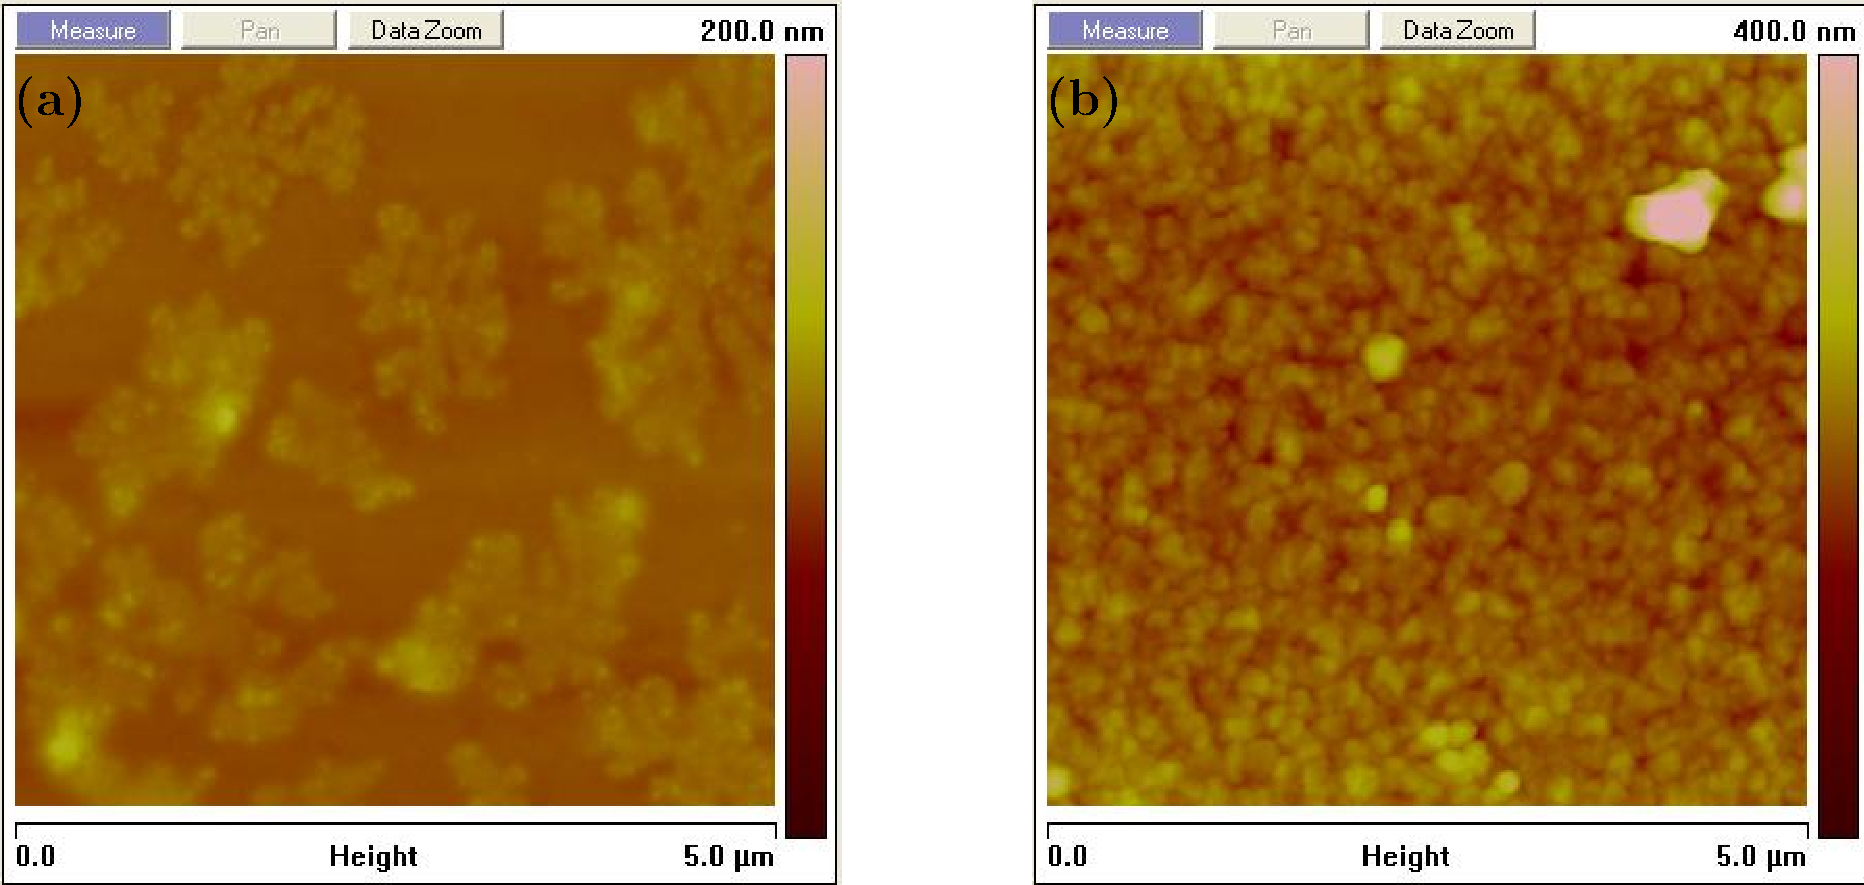
\includegraphics[width=0.8\textwidth]{figs/active/out/AFM.pdf}
 \caption[AFM pictures of silver deposited onto glass plates]{AFM pictures of silver deposited onto glass plates. \textbf{(a)} Flakes of silver oxide seem to be forming onto the deposited
	  silver layer. \textbf{(b)} Sample image showing the inhomogeneity of the
	  silver layer.}
 \label{fig:antenna.AFM}
\end{figure}


\paragraph*{Size Effects}
It has recently come to our attention that the conductivity 
of thin metal films can be a function of their thicknesses. 
We will explore this in future work, so for now 
suffice it to say that the Fuchs-Sondheimer model states
that
  \begin{equation}
      \sigma_F = \frac{\sigma_0}{1+\frac{3\lambda}{8d}\left(1-p\right)}
  \end{equation}
where $0\leq p\leq1$ is a specularity parameter and $\lambda$ is the 
electron free mean path in the metal. This model states that conductivity
diminishes as the thickness of the metallic layer gets smaller.


In Figure \ref{fig:antenna.thicknessRatios}, we compare the 
thicknesses obtained via the bulk conductivity model (Bruggeman 
effective conductivity) and the Fuchs-Sondheimer model with 
effective conductivity for the RF33 fibre. Given that the AFM pictures
show surface inhomogeneity, we assume diffuse scattering in 
the FS model ($p=0$). We see that chosing a dimensionality 
of 3 or 2 does not significantly affect the thicknesses, but
we see a difference of about 20\% in the effective conductivities.

The most interesting thing, though, is that the FS
model predicts metallic layers that are 10\% to 80\% thicker 
than with the bulk conductivity model. This will be explored 
in the next report. 

\begin{table}
  \newcolumntype{d}{D{.}{.}{3}}
  \caption[Geometric and physical parameters of the \gls{lcx} antennae]
	  {Geometric and physical parameters of the \gls{lcx} antennae.
	  Units are repeated from column above if not indicated.}
 \begin{subtable}[t]{0.45\textwidth}
 \caption[Geometric parameters of the RF21/RF33 fibre designs]
	  {Geometric parameters of the RF21/RF33 fibre designs. 
	  The thicknesses of the layers are listed in order, stating
	  from the inner layer to the outer layer of the fibre-antenna.}
 \label{tab:antenna.rfxx-parameters}
 \begin{tabular*}{\textwidth}{l@{\extracolsep{\fill}}c@{\extracolsep{\fill}}d@{\extracolsep{\fill}}d}
  \hline\hline
  Quantity			& Unit			& \multicolumn{1}{c}{RF21} 	& \multicolumn{1}{c}{RF33}	\\
  \hline
  $t_\text{vac}$		& $\unit{\mu m}$	& 99.874			& 99.924			\\
  $t_\text{Ag1}$		& 			& 0.126				& 0.0766			\\
  $t_\text{Si}$			& 			& 273				& 273				\\
  $t_\text{pyamide}$		& 			& 24				& 24				\\
  $t_\text{Ag2}$		& 			& 0.101				& 0.030				\\
  $d_L$				& $\unit{mm}$		& 27				& 30.91				\\
  $d_R$				& 			& 55				& 54.72				\\
  $S_{z1}$\parnote{Each window has a different $S_z$ and $d_z$.}
				& 			& 32				& 34.36				\\
  $S_{z2}$			& 			& 32				& 34.06				\\
  $S_{z3}$			& 			& 32				& 33.87				\\
  $d_{z1}$			& 			& 28				& 27.44				\\
  $d_{z2}$			& 			& 28				& 28.36				\\
  $L$				& $\unit{cm}$		& 30.0				& 24.372			\\
  $\theta_w$			& $\unit{deg}$		& 180				& 180				\\
  $R_\text{inner}$		& $\unit{\Omega}$	& 60.0				& 80.5				\\
  $R_\text{outer}$		&			& 20.0				& 59.8				\\
  \hline\hline
 \end{tabular*}
 \begin{flushleft}
 \parnotes
 \end{flushleft}
 \end{subtable}\hfill
 \begin{subtable}[t]{0.45\textwidth}
  \begin{center}
 \caption{Physical parameters of the materials used in the RF21/RF33 antennas.}
 \label{tab:antenna.physicalParameters}
 \begin{tabular*}{\textwidth}{l@{\extracolsep{\fill}}c@{\extracolsep{\fill}}d}
  \hline\hline
  Quantity			& Unit			& \multicolumn{1}{c}{Value}		\\
  \hline
  $\epsilon_\text{Si}$		& --			& 3.77		\\
  $\epsilon_\text{pyamide}$	& --			& 3.50		\\
  $\sigma_\text{Ag0}$		& $\unitfrac{MS}{m}$	& 63.0		\\
  $\sigma_\text{AgO0}$		& 			&  6.79		\\
  $\lambda_\text{Ag}$		& $\unit{nm}$		& 40		\\
  \hline\hline
 \end{tabular*}
 \begin{flushleft}
 \parnotes
 \end{flushleft}
 \end{center}
 \end{subtable}
\end{table}


\begin{figure}
  \centering
  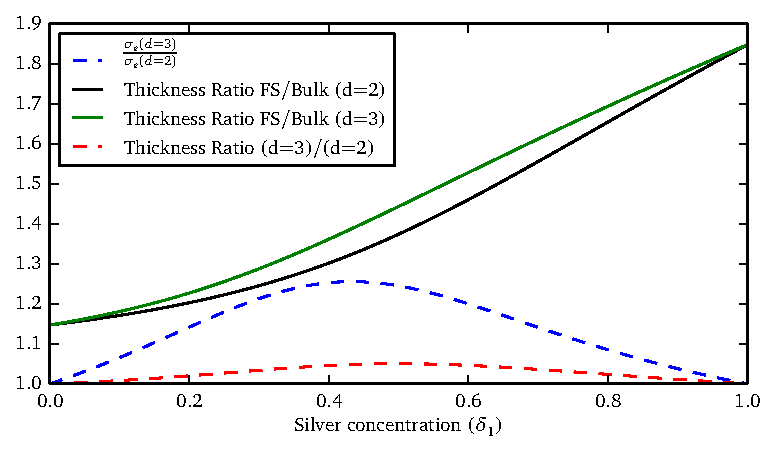
\includegraphics[width=0.9\textwidth]{figs/active/comparisonThickness.pdf}
  \caption[Thickness ratios as a function of the silver concentration]
	  {We show multiple ratios as a function of the silver concentration,
	  $\delta_1$. The blue line shows the ratio between the effective
	  conductivities for a choice of $d=2$ and $d=3$. The black and 
	  green lines show the ratio of the thickness predicted by using
	  the Fuchs-Sondheimer conductivity in Eq. \eqref{eq:antenna:thickGeneralEquations}
	  to the thickness predicted by using the bulk conductivity.
	  The red line shows the ratio of the green line to the black line.}
  \label{fig:antenna.thicknessRatios}
\end{figure}


\subsubsection{Finite Element Method}
As finite element methods directly solve Maxwell's equations, 
they can be a useful tool to verify semi-analytical methods. 
In the last report, we reported some agreement issues 
between experimental and simulation data. We purported
that the discrepancy was due to the small size of the
silver layers that we could properly account for in 
the finite element model. This issue has been solved
by abandoning the idea of properly meshing the silver layers
and replacing them by appropriate impedance boundary conditions.
From HFSS's documentation, we see that the ``Layered Impedance 
Boundary Conditions'' module follows the theory set forth in 
\cite{MIT1968} and others. 

We have simulated the RF21 fibre using Bruggeman's model
for the effective conductivity and with values
of $\delta_1\in\{0,1\}$ and $d=3$ in \eqref{eq:antenna:bruggeman}.
After obtaining the simulated $S_\text{11}$ parameter of the fibre,
we compared it to the experimentally obtained one using the Pearson
correlation coefficient. For two samples $\{X_i\}$ and 
$\{Y_i\}$, it is defined as
  \begin{equation}
    r = \frac{\sum_i^n\left(X_i-\left\langle X\right\rangle\right)\left(Y_i-\left\langle Y\right\rangle\right)}
	     {\sqrt{\sum_i^n\left(X_i-\left\langle X\right\rangle\right)^2}\sqrt{\sum_i^n\left(Y_i-\left\langle Y\right\rangle\right)^2}}.
  \end{equation}
From the definition, we see that the simultaneous linear transformations $X_i\rightarrow b+aX_i$ and $Y_i\rightarrow d+cY_1$
do not change the value of the Pearson coefficient. This means that even if the two samples
do not have the same normalization or are shifted by a constant amount, the correlation 
will stay the same. As such, the Pearson correlation measures the delegend(loc=1, prop={'size':6})
gree at which 
both samples are linearly related. 

Figure \ref{fig:antenna.sParameters} shows the experimental and simulated
$S_{11}$ parameter. At first look, it might seem like the general form 
of the curves are similar, but our quantitative analysis will show 
that that would be wrong. To make sure that our simulation data was not simply
shifted in frequency due to an small error in the geometry, we have
also calculated the correlation for a shifted dataset 
\footnote{To do so, we simply right-shifted the arrays containing
the simulation data and removed the data that fell outside the frequency range 
of the experimental data.}. This changes
the Pearson correlation because we must elide some of the experimental
and simulation data to do so. Figure \ref{fig:antenna.shiftCorrelation}
shows our results. We see that there are little to no correlation
between the simulation data and the experimental data with $r\in\{-0.04,0.05\}$. 

A possible source of error is the thickness of the silver layers. We will incorporate
the FS model in the next simulations and determine if it is
a factor. 

\begin{figure}
 \centering
 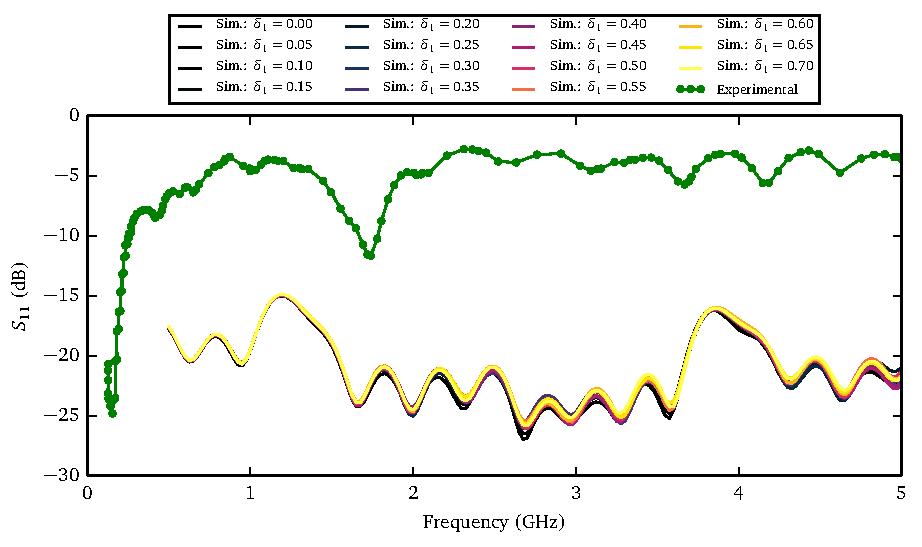
\includegraphics[width=0.8\textwidth]{figs/active/sParameters-concSweepS11.pdf}
 \caption[Experimental and simulated $S_{11}$ parameter for the RF21 fibre]
	 {Experimental and simulated $S_{11}$ parameter for the RF21 fibre.}
 \label{fig:antenna.sParameters}
\end{figure}

\begin{figure}
 \centering
 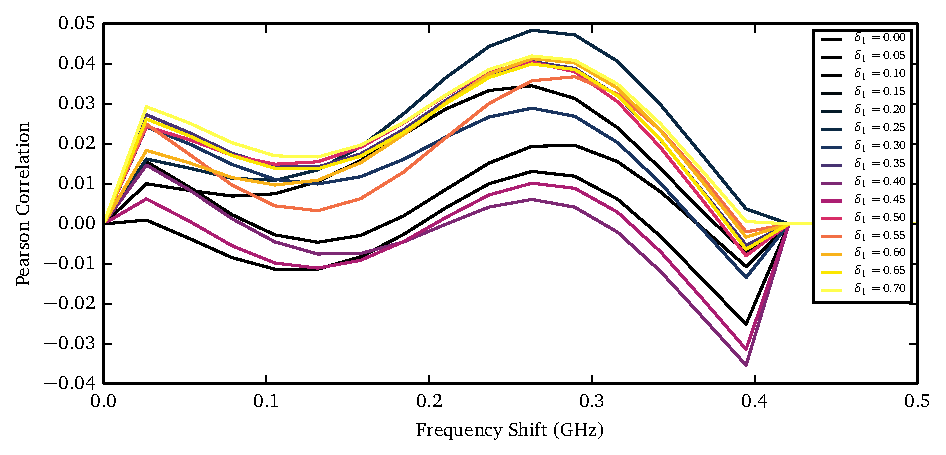
\includegraphics[width=0.8\textwidth]{figs/active/shiftCorrelationS11.pdf}
 \caption{Pearson correlation coefficient as a function of the frequency
	  shift of the data.}
 \label{fig:antenna.shiftCorrelation}
\end{figure}

We have also taken the Fourier transform of the experimental
and simulation data (for $\delta_1=0$). To our discontent, 
it seems that the datasets do not share periodic properties. 
Figure \ref{fig:antenna.fourierAnalysis} shows the intensity
of the FFT transform. To see if the periodic components corresponded
to particular lengths in the system, we converted the associated
wavelenghts to frequencies and plotted them as vertical lines in the figure. 
$f_1$ is the fundamental mode of infinite LCXF, namely
  \begin{equation}
   f_1 = \frac{c}{\left(S_z+d_z\right)\left(\sqrt{\epsilon_\text{Si}}+1\right)}.
  \end{equation}
The frequency associated with the optical and the actual lengths of the window
are
  \begin{align*}
   l_\text{opt}	&= \frac{c}{S_z\sqrt{\epsilon_\text{Si}}}	\\
   l_\text{phy}	&= \frac{c}{S_z}.
  \end{align*}

Nothing thus far seems to explain the periodic properties of the 
$S_{11}$ parameter of the experimental and simulation, although
the optical length of the windows seems to explain a single 
peak in the Fourier power spectrum. 

The author is not sure that is the proper method to
analyze the Fourier spectrum, however. 

\begin{figure}
 \centering
 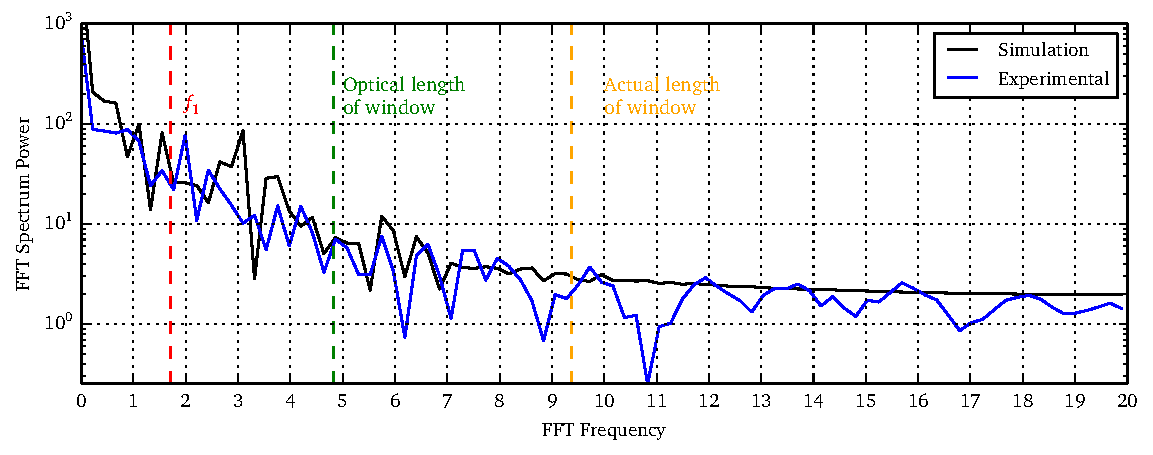
\includegraphics[width=0.8\textwidth]{figs/active/fourierAnalysisS11.pdf}
 \caption[Fourier Power Spectrum]
	  {Absolute value of the Fourier transform of the $S_{11}$ parameter.
	  The red lines denote the frequencies associated with certain lengths
	  in the RF21 fibre design.}
 \label{fig:antenna.fourierAnalysis}
\end{figure}
